% !TeX spellcheck = pl_PL
\documentclass[a4paper]{article}
\usepackage{polski}
\usepackage[utf8]{inputenc}
\usepackage{graphicx}
\usepackage{amsmath}

\usepackage[unicode, bookmarks=true]{hyperref} %do zakładek
\usepackage{tabto} % do tabulacji
\NumTabs{6} % globalne ustawienie wielkosci tabulacji
\usepackage{array}
\usepackage{multirow}
\usepackage{array}
\usepackage{dcolumn}
\usepackage{bigstrut}
\usepackage{color}
\usepackage[usenames,dvipsnames]{xcolor}
\usepackage{wrapfig}
\usepackage{listings,lstautogobble}
\usepackage[usenames,dvipsnames]{xcolor}
\usepackage{titlesec}

\makeatletter
\@addtoreset{section}{part}
\makeatother

\setlength{\textheight}{24cm}
\setlength{\textwidth}{15.92cm}
\setlength{\footskip}{10mm}
\setlength{\oddsidemargin}{0mm}
\setlength{\evensidemargin}{0mm}
\setlength{\topmargin}{0mm}
\setlength{\headsep}{5mm}
\newcommand{\HRule}{\rule{\linewidth}{0.5mm}}
\usepackage{endnotes}
\def\enoteheading{\par\kern2\baselineskip%
	\footnoterule%
	\kern1\baselineskip}
\let\footnote\endnote
\def\footnotetext{\endnotetext[\number\numexpr\value{endnote}+1]}
\let\footnotemark\endnotemark 

% --- Opcje listingu kodu
\lstset{
	frame=single,
	autogobble=true,
	commentstyle=\ttfamily\itshape\color{ForestGreen},
	keywordstyle=\color{blue},
	frameround=ffff,
	rulecolor=\color{black},
	tabsize=4,
	breaklines=true, %
	% --- Polskie znaki w listingu kodu
	literate=%
	{ą}{{\c{a}}}1
	{ć}{{\'c}}1
	{ę}{{\c{e}}}1
	{ł}{{\l{}}}1
	{ń}{{\'n}}1
	{ó}{{\'o}}1
	{ś}{{\'s}}1
	{ź}{{\'z}}1
	{ż}{{\.z}}1
	{Ą}{{\c{A}}}1
	{Ć}{{\'C}}1
	{Ę}{{\c{E}}}1
	{Ł}{{\L{}}}1
	{Ń}{{\'N}}1
	{Ó}{{\'O}}1
	{Ś}{{\'S}}1
	{Ź}{{\'Z}}1
	{Ż}{{\.Z}}1
}
% -- listing SiSzarpa
\definecolor{bluekeywords}{rgb}{0,0,1}
\definecolor{greencomments}{rgb}{0,0.5,0}
\definecolor{redstrings}{rgb}{0.64,0.08,0.08}
\definecolor{xmlcomments}{rgb}{0.5,0.5,0.5}
\definecolor{types}{rgb}{0.17,0.57,0.68}
\lstset{
	language=[Sharp]C,
	captionpos=b,
	%numbers=left, %Nummerierung
	%numberstyle=\tiny, % kleine Zeilennummern
	frame=lines, % Oberhalb und unterhalb des Listings ist eine Linie
	showspaces=false,
	showtabs=false,
	breaklines=true,
	showstringspaces=false,
	breakatwhitespace=true,
	escapeinside={(*@}{@*)},
	commentstyle=\color{greencomments},
	morekeywords={partial, var, value, get, set, Double, DateTime},
	keywordstyle=\color{bluekeywords},
	stringstyle=\color{redstrings},
	basicstyle=\ttfamily\small,
}

\usepackage{titlesec}

\begin{document}
\bibliographystyle{plain}

	\begin{titlepage}
		\begin{center}
			
			% Upper part of the page. The '~' is needed because \\
			% only works if a paragraph has started.
			
\includegraphics[width=0.5\textwidth]{./img/logo.png}~\\[1cm]
			%?[width=0.15\textwidth]
			
			\textsc{\LARGE Politechnika Śląska w Gliwicach}\\[1.5cm]
			
			\textsc{\Large Biologically Inspired Artificial Intelligence}\\[0.5cm]
			
			% Title
			\HRule \\[0.4cm]
			{ \huge \bfseries Przewidywanie kursu walutowego  \\[0.4cm] }
			
			\HRule \\[1.5cm]
			
			% Author and supervisor
			\textsc{\Large Autorzy:} \\
			Forczmański Mateusz \\
			Szukała Patryk\\[1.0cm]
			
			Informatyka, semestr VI \\
			Rok akademicki 2014/2015 \\
			Grupa GKiO3
			
			\vfill
			
			% Bottom of the page
			{\large \today}
			
		\end{center}
	\end{titlepage}
	{\hypersetup{hidelinks}
		\tableofcontents
	}
	\newpage
	
	\part{Temat projektu}
		\section{Cel zadania}
		Naszym zadaniem było przewidywanie kursu walutowego EUR/USD (euro / dolar) na rynku Forex. W założeniach naszego projektu mieliśmy wykonać je na sieciach neuronowych.\\
		Idea przewidywania kursu walutowego polega na analizie danych historycznych kursu oraz trendu, jakim wykres kursu zmierza. Celem naszego programu jest takie wytrenowanie sieci neuronowej, aby sama mogła przewidzieć przyszły kursy. Wartości te są niezwykle zmienne w czasie i trudne do przewidzenia, a w profesjonalnym oprogramowaniu, gdy  prawdopodobieństwo prawidłowego oszacowania przyszłego kursu przekracza 60\% , jest to uznawane za sukces. Korzyścią takiego programu jest oczywiście ułatwienie podejmowania decyzji finansowych.
		\section{Analiza problemu}\label{sec:analiza}
			Wartości kursów na rynku Forex zmieniają się z dokładnością co do sekund (tzw. \emph{tick}, który nie ma stałej wartości). By móc uprościć nasze zadanie zdecydowaliśmy się pobierać dane z dokładnością co do \textit{dnia}. W tej jednostce można wyróżnić 4 wartości kursu:
			\begin{itemize}
				\item \textbf{Open} - wartość otwarcia danego dnia
				\item \textbf{Low} - minimalna wartość w ciągu dnia
				\item \textbf{High} - maksymalna wartość w ciągu dnia
				\item \textbf{Close} - wartość zamknięcia danego dnia
			\end{itemize}
			Te cztery wartości z każdego dnia stanowią nasze dane wejściowe. Nie są to również jedyne parametry, które określają wartość kursu. Zdecydowaliśmy się naszej sieci przekazywać również współczynnik \textbf{RSI}\,(\emph{Relative Strength Index}), który określa siłę trendu. Oblicza się go w następujący sposób:
			$$ RSI=1-\cfrac{1}{1+\cfrac{A_k}{B_k}}$$
			gdzie:
			\begin{itemize}
				\item $ A_k $ - średnia wartość wzrostu cen zamknięcia z \textit{k} dni
				\item $ B_k $ - średnia wartość spadku cen zamknięcia z \textit{k} dni
			\end{itemize}
		\section{Wynik obliczeń}
			Nasza sieć decyduje czy wartość kursu zamknięcia następnego dnia będzie większa lub mniejsza od kursu zamknięcia dnia dzisiejszego. Zwrócona przez sieć wartość interpretowana jest następująco:
			\begin{itemize}
				\item $ 0 $ - wartość kursu będzie mniejsza
				\item $ 1 $ - wartość kursu będzie większa
			\end{itemize}
		\newpage
	\part{Specyfikacja zewnętrzna}
		\section{Interfejs graficzny}
			\begin{figure}[h!]
				\centering
				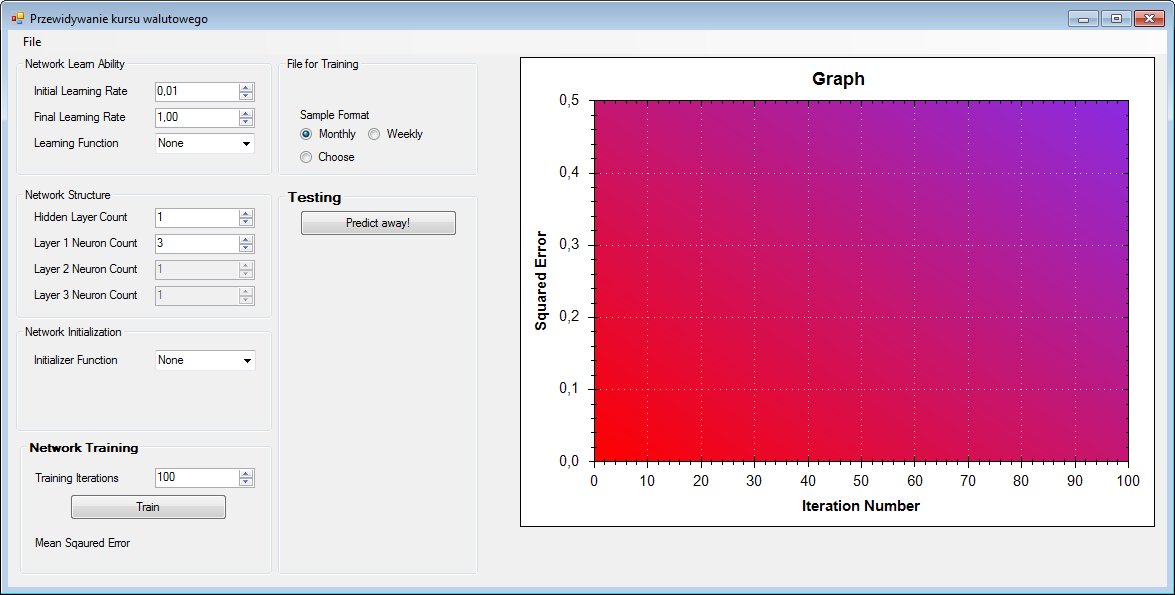
\includegraphics[width=0.90\textwidth]{./img/GUI}
				\caption{Interfejs po uruchomieniu programu}
			\end{figure}
			Przed przystąpieniem do trenowania sieci można są skonfigurować:
			\subsection{Struktura sieci}
				\begin{figure}[h!]
					\centering
					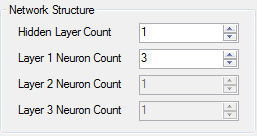
\includegraphics[width=0.40\textwidth]{./img/GUI_network_structure}
					\caption{Panel do konfiguracji struktury sieci z domyślnymi wartościami}
				\end{figure}
				W tym panelu definiuje się budowę wewnętrzną sieci neuronowej - liczbę warstw pośrednich oraz liczbę neuronów w każdej z warstw. Maksymalnie można utworzyć 3 warstwy z minimum 1 neuronem. W zależności od wartości w polu \emph{Hidden Layer Count}, odpowiednie pola \emph{Layer Neuron Count} są dostępne lub nie.
			\newpage
			\subsection{Zdolność nauki}
				\begin{figure}[h!]
					\centering
					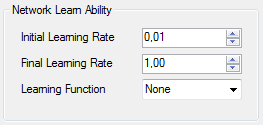
\includegraphics[width=0.40\textwidth]{./img/GUI_initial_learning}
					\caption{Panel do konfiguracji zdolności nauki z domyślnymi wartościami}
				\end{figure}
				Ten panel znajduje się w górnym lewym rogu interfejsu. Umożliwia konfigurację trzech parametrów:
				\begin{itemize}
					\item \emph{Initial Learning Rate} - wartość startowa zdolności nauki, z nią uruchamiany jest trening sieci.
					\item \emph{Final Learning Rate} - wartość zdolności nauki, którą sieć będzie miała, gdy trening się skończy.
					\item \emph{Learning Function} - specjalizowana funkcja, jakiej sieć backpropagacji będzie wykorzystywać do nauki. Są cztery możliwości:
					\begin{itemize}
						\item \emph{None} - standardowa funkcja
						\item \emph{Expotential} - funkcja eksponencjalna
						\item \emph{Hyperbolic} - funkcja hiperboliczna
						\item \emph{Linear} - funkcja liniowa
					\end{itemize}
				\end{itemize}
			\subsection{Inicjalizacja funkcji}
				\begin{figure}[h!]
					\centering
					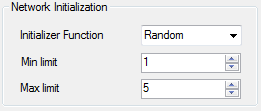
\includegraphics[width=0.40\textwidth]{./img/GUI_network_initialization}
					\caption{Panel do konfiguracji inicjalizacji sieci z przykładowymi ustawieniami}
				\end{figure}
				W tej części (lewa strona interfejsu) można ustawić inicjalizację sieci, czyli początkową wartość wag neuronów we wszystkich warstwach. Istnieje cześć możliwości:
				\begin{itemize}
					\item \emph{None} - wartości domyślne.
					\item \emph{Constant} - wskazana wartość stała.
					\item \emph{NgyuenWidrow} - sparametryzowana funkcja\textit{ NGuyen Widrow}.
					\item \emph{NormalizedRandom} - znormalizowana wartość losowa.
					\item \emph{Random} - wartość losowa ze wskazanego zakresu.
					\item \emph{Zero} - funkcja typu Zero (wszystkie wartości są zbliżone do zera).
				\end{itemize}
			\newpage
			\subsection{Analiza plików}
				\begin{figure}[h!]
					\centering
					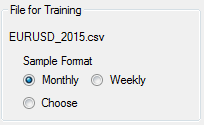
\includegraphics[width=0.40\textwidth]{./img/GUI_files}
					\caption{Panel z wczytanym plikiem i sposobem podziału}
				\end{figure}
				Ten panel znajduje się w górnej środkowej części interfejsu. Umożliwia pogląd załadowanego pliku do treningu sieci (tutaj \textit{EURUSD\_2015.csv}) oraz sposób w jaki dane będą grupowane:
				\begin{itemize}
					\item \emph{Monthly} - co miesiąc.
					\item \emph{Weekly} - co tydzień.
					\item \emph{Choose} - wg wskazanej przez użytkownika liczby dni.
				\end{itemize}
			\subsection{Trening sieci}
				\begin{figure}[h!]
					\centering
					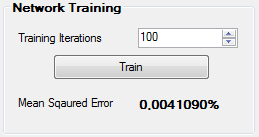
\includegraphics[width=0.40\textwidth]{./img/GUI_network_training}
					\caption{Przykładowy wynik trenowania sieci po 100 iteracjach}
				\end{figure}
				Ten panel znajduje się w dolnym prawym rogu. Wymaga od użytkownika wprowadzania liczby iteracji treningowych, jakie wykona sieć (domyślnie jest to wartość 100). Po wciśnięciu przycisku \emph{Train} sieć rozpocznie swój trening. Gdy zostanie on zakończony, na dole pojawia się \emph{Mean Sqaured Error} (średni kwadratowy błąd) sieci w procentach. Oznacza on jakie wg obliczeń jest prawdopodobieństwo błędu sieci, czyli złego przewidzenia linii trendu kursu waluty.\\
				Program poświęca 70\% próbek (zaokrąglonych w górę) do testów.
			\newpage
			\subsection{Trening sieci}
				\begin{figure}[h!]
					\centering
					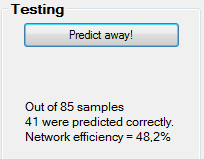
\includegraphics[width=0.30\textwidth]{./img/GUI_testing}
					\caption{Przykładowy wynik testowania sieci}
				\end{figure}
				Na środku interfejsu znajduje się przycisk \emph{Predict away!}. Gdy sieć została wytrenowana i skonfigurowana, jego wciśnięcie powoduje uruchomienie testowania sieci i zmierzenie jej efektywności. Po wykonaniu testów informacje zostaną wyświetlone w tym samym panelu.\\ Program poświęca 30\% próbek w celu zbadania jakości działania sieci.
			\subsection{Graf błędu}
				\begin{figure}[h!]
					\centering
					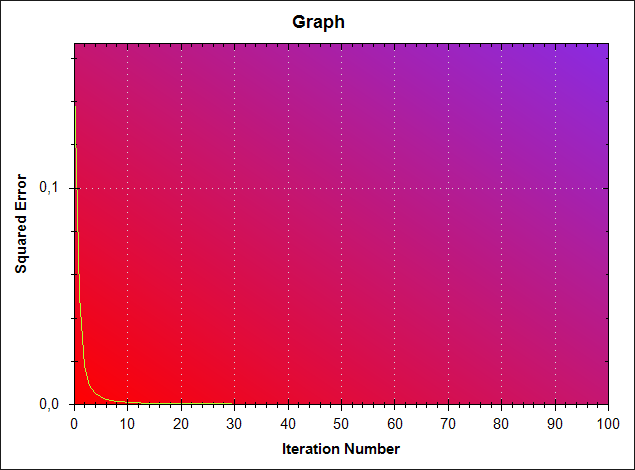
\includegraphics[width=0.85\textwidth]{./img/GUI_graph}
					\caption{Przykładowy przebieg nauki sieci}
				\end{figure}
				W czasie treningu sieci jest generowany graf zależności jakości sieci od liczby iteracji. Przedstawia on jak prawdopodobieństwo błędu zmieniało się wraz z kolejnymi iteracjami. Można powiedzieć, że obrazuje on, w jaki sposób sieć się uczy.\\
				Maksymalną wartością na osi poziomej jest liczba iteracji, z kolei na osi pionowej jest to maksymalny średni błąd kwadratowy (wyliczany dynamicznie w trakcie działania programu).
		\section{Korzystanie z programu}
			Aby móc wytrenować sieć i badać jej efekty, wystarczy wykonać kilka prostych kroków:
			\begin{enumerate}
				\item Wczytać plik z danymi próbkowymi. Należy wybrać z górnego menu \textit{File}$ \rightarrow $\emph{Open} i wskazać odpowiedni plik CSV.
				\item Ustawić wszystkie parametry zgodnie z instrukcjami w poprzednim podrozdziale.
				\item Wybrać \emph{Train} by wytrenować sieć.
				\item Wybrać \emph{Predict away!} by testować sieć.
			\end{enumerate}
	\part{Wykonanie i specyfikacja wewnętrzna}
		\section{Dane testowe}
			\subsection{Zbieranie}
				By móc przystąpić do działania, potrzebowaliśmy danych historycznych o kursie EUR/USD na rynku Forex. Istnieje dużo stron, które udostępniają te dane za odpowiednią opłatą, ale nie chcąc ani wydawać dziesiątek dolarów za nie, ani zakładać własnej firmy, szukaliśmy źródła, które udostępniłoby dane za darmo i przyjaznym formacie. Ostatecznie znaleźliśmy dwie strony internetowe, które nam pomogły:
				\begin{itemize}
					\item \url{http://www.global-view.com/forex-trading-tools/forex-history/} - strona za darmo udostępnia dane historyczne na temat kursu EUR/USD w formacie CSV. W generowanych przez nią plikach, z dokładnością do dnia, znajdują się kursy zamknięcia, najwyższy oraz najniższy w ciągu dnia. Prawie idealnie spełniało to nasze potrzeby.
					\item \url{http://pl.investing.com/currencies/eur-usd-historical-data} - strona za darmo wyświetla dane historyczne w postaci tabeli, której dane można kopiować. Mając dane z poprzedniej strony, wszystkie potrzebne nam wartości dziennych kursów otwarcia kopiowaliśmy ręcznie do pliku CSV.
				\end{itemize}
			\subsection{Format pliku}\label{subsec:format}
				Postanowiliśmy, żeby format pliku wejściowego był jak najprostszy, by dane mogły być szybko przetworzone, a jednocześnie wygodnie uzupełniane w miarę rozrastania się pliku. Zachowaliśmy plik CSV, jaki dostarczyła jedna ze stron, jest on wygodny oraz łatwy do sparsowania.\\
				Przykładowy kawałek pliku:
				\begin{lstlisting}
					2014-01-01,1.3745,1.3754,1.3744,1.38004
					2014-01-02,1.3655,1.3775,1.3627,1.37629
					2014-01-03,1.3587,1.3672,1.3583,1.36664
					2014-01-06,1.3634,1.3653,1.3569,1.35908
					2014-01-07,1.3614,1.366,1.3594,1.36289
					2014-01-08,1.3581,1.3635,1.3551,1.36153
				\end{lstlisting}
				Data stanowi unikalny klucz dziennego kursu i nie może się powtarzać. W tym rodzaju pliku nagłówki są zbędne, więc aby móc łatwo zapamiętać, która wartość jest która, ułożyliśmy je \textit{alfabetycznie}. Plik kolejno przedstawia:
				\begin{center}
					Data, \textbf{C}lose (zamknięcie), \textbf{H}igh (maksymalny), \textbf{L}ow (minimalny), \textbf{O}pen (otwarcie)
				\end{center}
			\subsection{Parsowanie pliku}
				Ponieważ istnieje spora liczba gotowych bibliotek do parsowania plików CSV, zdecydowaliśmy się nie pisać własnej funkcji, tylko skorzystać z jednej z już istniejących. Nie szukaliśmy długo, nasz wybór padł na małą, ale bardzo wysoko ocenianą bibliotekę "CSV Parser" autorstwa Ideafixxxer (prawdziwe imię i nazwisko nieznane) ze strony Code Project\footnote{Parser CSV: \url{http://www.codeproject.com/Tips/741941/CSV-Parser-Csharp}}.\\
				Biblioteka przyjmuje na wejście plik CSV oraz zwraca strukturę typu \textbf{\color{blue}{string}[][]} z informacjami z pliku CSV w postaci tekstu. Format ten nie jest dogodny dla naszych potrzeb, dlatego napisaliśmy własny kod, który zmienia ową tablicę dwuwymiarową na mapę: kluczem jest data, a wartością tablica jednoelementowa wartości typu \textbf{\color{blue}{double}}. Całość została zakapsułkowana do klasy \emph{ExchangeData}. Co prawda po formacie próbek wyraźnie widać, że wystarczyłby typ danych \textbf{\color{blue}{float}}, jednak nasza biblioteka przyjmuje jako parametry wartości \textbf{\color{blue}{double}}, więc postanowiliśmy poświęcić tych kilka kilobajtów by uniknąć konieczności wielokrotnego rzutowania.
				\begin{lstlisting}
					class ExchangeData
					{
						private const int RATE_NUMBER = 4;
						private readonly Dictionary<DateTime, Double[]> data;
						
						public ExchangeData(string[][] inputData)
						{
							data = new Dictionary<DateTime, Double[]>();
							for (int i = 0; i < inputData.GetLength(0); i++)
							{
								DateTime dt = ToDateTime(inputData[i][0]);
								Double[] rate = new Double[RATE_NUMBER];
								// Close
								rate[0] = Double.Parse(inputData[i][1], CultureInfo.InvariantCulture);
								// High
								rate[1] = Double.Parse(inputData[i][2], CultureInfo.InvariantCulture);
								// Low
								rate[2] = Double.Parse(inputData[i][3], CultureInfo.InvariantCulture);
								// Open
								rate[3] = Double.Parse(inputData[i][4], CultureInfo.InvariantCulture);
								this.data[dt] = rate;
							}
						}
						
						public static DateTime ToDateTime(string datetime)
						{
							string year = datetime.Substring(0, 4);
							string month = datetime.Substring(5, 2);
							string day = datetime.Substring(8, 2);
							return new DateTime(Convert.ToInt32(year), Convert.ToInt32(month), Convert.ToInt32(day));
						}
					};
				\end{lstlisting}
	\theendnotes
	\newpage
	\section{Obliczanie współczynnika RSI}
	\begin{lstlisting}
	private double calculateRSI(List<Double[]> input, int start = 0)
	{
		int periodNumber = input.Count - start;
		double alpha = 2.0d / (periodNumber + 1);
		double denominator = 0.0d;
		double avg_growth = 0.0d, avg_fall = 0.0d;
		List<double> growth = new List<double>();
		List<double> fall = new List<double>();
		// porównanie wartości Close pomiędzy kolejnymi dniami oraz obliczenie spadku/wzrostu
		for (int i = start; i < periodNumber - 1; ++i)
		{
			double weight = Math.Pow(1 - alpha, periodNumber - i);
			double value = input[i][0];
			double value_next = input[i + 1][0];
			if ((value - value_next) >= 0)
				fall.Add((value - value_next) * weight);
			else
				fall.Add(0);
			if ((value_next - value) >= 0)
				growth.Add((value_next - value) * weight);
			else
				growth.Add(0);
			denominator += weight;
		}
		//obliczanie sredniego spadku/wzrostu
		avg_fall = fall.Sum() / denominator;
		avg_growth = growth.Sum() / denominator;
		//oblicznie RSI
		double RSI = 100 - (100 / (1 + (avg_growth / avg_fall)));
		return RSI;
	}
	\end{lstlisting}
	Metoda zwracająca współczynnik RSI (patrz: Analiza Problemu \ref{sec:analiza}). W celu obliczenia średniego wzrostu i spadku kursu wykorzystano pętle, która iteruje po podanej liście zawierającej dane historyczne kursów (parametr \emph{input}). Zależnie od tego czy różnica między wartością Close aktualnego dnia, a dnia następnego jest dodatnia czy ujemna, następuje dodanie tej różnicy do odpowiedniej listy (spadków / wzrostów). W przypadku wartości spadku różnica obliczana jest między dniem następnym, a aktualnym, po to aby wartości w obu listach były dodatnie.\\
	W ciele funkcji odnosimy się do elementu zerowego tablicy, ponieważ właśnie tam znajdują się kursy zamknięcia (patrz: format pliku \ref{subsec:format}).\\
	Po wyjściu z pętli następuje obliczenie średnich z wartości znajdujących się w listach, a następnie podstawienie tych wartości do wzoru (patrz: Analiza Problemu \ref{sec:analiza}) i zwrócenie jej przez metodę.
	
\end{document}